\documentclass[11pt,a4paper]{article}
\usepackage[T1]{fontenc}
\usepackage[utf8]{inputenc}
\usepackage{lmodern,microtype,textcomp,amsmath,amssymb}
\usepackage[margin=2.2cm]{geometry}
\usepackage{booktabs,tabularx,array,caption,enumitem,graphicx}
\usepackage{xcolor}
\usepackage{tikz}
\usetikzlibrary{shapes.geometric,arrows.meta,positioning}
\usepackage[colorlinks=true,linkcolor=black,urlcolor=blue!60!black]{hyperref}
\setlength{\parindent}{0pt}
\setlength{\parskip}{0.55em}
\definecolor{upc}{HTML}{2E7D4F}
\definecolor{downc}{HTML}{B3403A}
\newcommand{\up}{\textcolor{upc}{$\blacktriangle$}}
\newcommand{\down}{\textcolor{downc}{$\blacktriangledown$}}
\newcolumntype{Y}{>{\raggedright\arraybackslash}X}
\newcolumntype{C}{>{\centering\arraybackslash}p{1.8cm}}
\captionsetup{font=small,labelfont=bf,skip=4pt}
\renewcommand{\arraystretch}{1.15}

\begin{document}

\begin{center}
{\LARGE\bfseries Retrieval-augmented QA over the articles of the Constitution of India}\par\vspace{0.6em}
{Achyutananda Sahoo \quad\textbullet\quad Reg.\ No.\ 2025202028}\par\vspace{0.3em}
{\small Code: \url{https://github.com/Sahoo-Achyutananda/theRAGofakind} (notebook: \texttt{rag.ipynb})}\par\vspace{0.1em}
{\small Dataset: \url{https://www.legislative.gov.in/constitution-of-india}}\par
\end{center}
\vspace{0.4em}

The Constitution of India consists of articles and schedules. The RAG is built on top of the articles alone; the schedules are not normal text and require additional preprocessing, and hence, for simplicity, were skipped for this assignment submission. The Constitution is complex and equally interesting. It also has its own set of contradictions (for example Art.~15(1) vs.\ 15(3), Art.~13(2) vs.\ 13(4), Art.~359 with its exception for Articles 20 and 21, and Art.~31 omitted with the right to property moved to Art.~300A), hence it fit well for this assignment, especially to analyze failure modes.

One caveat: the LLMs would have been trained on the Constitution, therefore the system prompt must specify to use only the chunks for answering these questions.

\section{Chunking}

\subsection{Text extraction with pdfplumber}
Normal text extraction includes the footnotes. To exclude the footnotes, a complex regex was required, and the regex worked for some pages but not for others. The articles and footnotes are separated by a horizontal line, and pdfplumber has its own codes defined for these graphical elements, hence pdfplumber was used.

\subsection{Splitting the text into articles}
An article here is the text between one article heading and the next; a regex was used to identify the headings. Articles contain clauses. Most articles fit within 1000 characters, and hence article-wise splitting was done. Longer articles are split at their clauses, and clauses that still exceed 1000 characters are split into multiple chunks at line breaks.

\subsection{Structure-aware chunking}
The maximum chunk size is 1000 characters. Figure~\ref{fig:chunkflow} shows the chunking flow used in the notebook.

There is no overlap, because most articles and article clauses fit into the 1000-character window; only the clauses split at line breaks (142 chunks) could have benefited from overlap.

\begin{center}
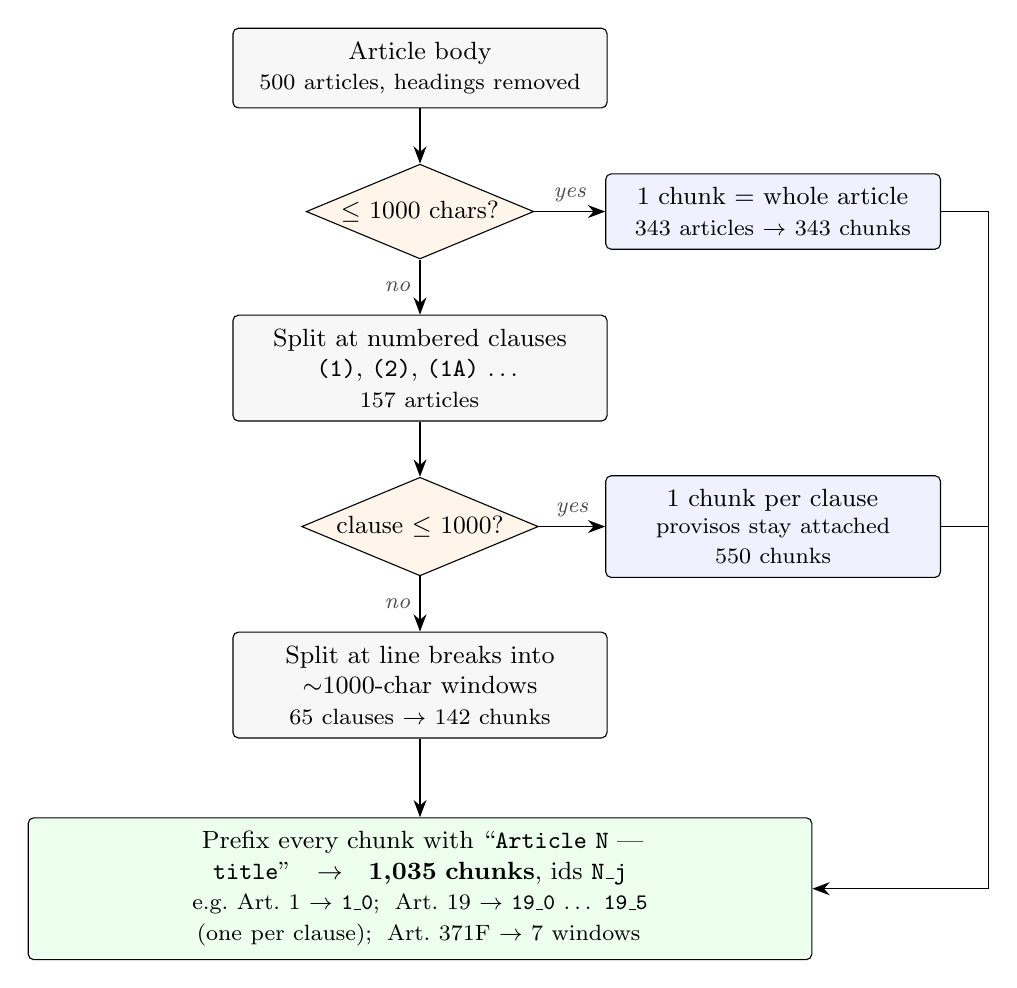
\begin{tikzpicture}[
    node distance=7mm and 9mm, >={Stealth[length=2.2mm]}, font=\small,
    box/.style={draw, rounded corners=2pt, fill=gray!6, align=center, inner sep=5pt, text width=4.4cm},
    outbox/.style={draw, rounded corners=2pt, fill=blue!6, align=center, inner sep=5pt, text width=3.9cm},
    dec/.style={draw, diamond, aspect=2.4, fill=orange!8, align=center, inner sep=1pt},
    lab/.style={font=\footnotesize\itshape, text=black!70}]
  \node[box] (in) {Article body\\{\footnotesize 500 articles, headings removed}};
  \node[dec, below=of in] (d1) {$\le$ 1000 chars?};
  \node[outbox, right=of d1] (whole) {1 chunk = whole article\\{\footnotesize 343 articles $\to$ 343 chunks}};
  \node[box, below=of d1] (clause) {Split at numbered clauses\\\texttt{(1)}, \texttt{(2)}, \texttt{(1A)} \ldots\\{\footnotesize 157 articles}};
  \node[dec, below=of clause] (d2) {clause $\le$ 1000?};
  \node[outbox] (cl) at (whole |- d2) {1 chunk per clause\\{\footnotesize provisos stay attached\\550 chunks}};
  \node[box, below=of d2] (win) {Split at line breaks into\\$\sim$1000-char windows\\{\footnotesize 65 clauses $\to$ 142 chunks}};
  \node[box, below=10mm of win, text width=9.6cm, fill=green!7] (pre)
       {Prefix every chunk with ``\texttt{Article N} --- \texttt{title}''\quad$\to$\quad\textbf{1,035 chunks}, ids \texttt{N\_j}\\
        {\footnotesize e.g.\ Art.\ 1 $\to$ \texttt{1\_0};\; Art.\ 19 $\to$ \texttt{19\_0} \ldots\ \texttt{19\_5} (one per clause);\; Art.\ 371F $\to$ 7 windows}};
  \draw[->] (in) -- (d1);
  \draw[->] (d1) -- node[lab, above] {yes} (whole);
  \draw[->] (d1) -- node[lab, left] {no} (clause);
  \draw[->] (clause) -- (d2);
  \draw[->] (d2) -- node[lab, above] {yes} (cl);
  \draw[->] (d2) -- node[lab, left] {no} (win);
  \draw[->] (win) -- (pre);
  \draw[->] (whole.east) -- ++(6mm,0) |- (pre.east);
  \draw (cl.east) -- ++(6mm,0);
\end{tikzpicture}
\captionof{figure}{Chunking flow used in \texttt{rag.ipynb}. Maximum body size 1000 characters ($\approx$ the bi-encoder's 256-token limit); with the prefix the longest chunk is 1,124 characters.}\label{fig:chunkflow}
\end{center}

\section{Architecture comparison: bi-encoder vs.\ cross-encoder}
\begin{itemize}[leftmargin=1.2em]
\item \textbf{Bi-encoder:} we pass the chunks and the query separately, and then find the cosine similarity.
\item \textbf{Cross-encoder:} we pass the query and the chunk attached together, for each chunk. The attention layer involves matching the tokens of the query and the chunk, making the ranking more accurate.
\item \textbf{Difference:} the latency of the cross-encoder is high, and hence it is only used for re-ranking. The bi-encoder extracts the top 10 chunks and passes them to the cross-encoder.
\end{itemize}

\par\medskip\noindent\begin{minipage}{\linewidth}\centering
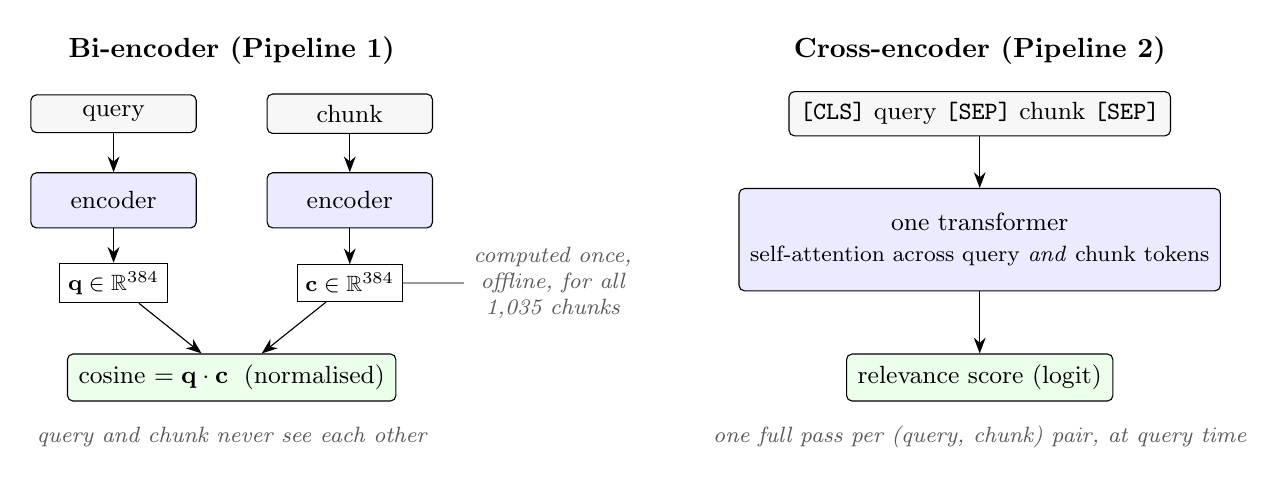
\begin{tikzpicture}[
    >={Stealth[length=2mm]}, font=\small,
    txt/.style={draw, rounded corners=2pt, fill=gray!6, align=center, inner sep=4pt, minimum width=2.1cm},
    enc/.style={draw, rounded corners=2pt, fill=blue!8, align=center, inner sep=4pt, minimum width=2.1cm, minimum height=7mm},
    vec/.style={draw, fill=white, align=center, inner sep=3pt, font=\footnotesize},
    sc/.style={draw, rounded corners=2pt, fill=green!8, align=center, inner sep=4pt},
    note/.style={font=\footnotesize\itshape, text=black!65, align=center}]
  \node[font=\bfseries] at (2.4,4.9) {Bi-encoder (Pipeline 1)};
  \node[txt] (q) at (0.9,4.1) {query};
  \node[txt] (c) at (3.9,4.1) {chunk};
  \node[enc] (eq) at (0.9,3.0) {encoder};
  \node[enc] (ec) at (3.9,3.0) {encoder};
  \node[vec] (vq) at (0.9,1.95) {$\mathbf{q}\in\mathbb{R}^{384}$};
  \node[vec] (vc) at (3.9,1.95) {$\mathbf{c}\in\mathbb{R}^{384}$};
  \node[sc] (cos) at (2.4,0.75) {cosine $=\mathbf{q}\cdot\mathbf{c}$ \;(normalised)};
  \draw[->] (q) -- (eq); \draw[->] (eq) -- (vq);
  \draw[->] (c) -- (ec); \draw[->] (ec) -- (vc);
  \draw[->] (vq) -- (cos); \draw[->] (vc) -- (cos);
  \node[note, anchor=west] (off) at (5.35,1.95) {computed once,\\offline, for all\\1,035 chunks};
  \draw[black!40] (vc.east) -- (off.west);
  \node[note] at (2.4,0.0) {query and chunk never see each other};
  \begin{scope}[xshift=9.5cm]
  \node[font=\bfseries] at (2.4,4.9) {Cross-encoder (Pipeline 2)};
  \node[txt, minimum width=4.6cm] (pair) at (2.4,4.1) {\texttt{[CLS]} query \texttt{[SEP]} chunk \texttt{[SEP]}};
  \node[enc, minimum width=4.6cm, minimum height=1.3cm] (tr) at (2.4,2.5) {one transformer\\{\footnotesize self-attention across query \emph{and} chunk tokens}};
  \node[sc] (s) at (2.4,0.75) {relevance score (logit)};
  \draw[->] (pair) -- (tr); \draw[->] (tr) -- (s);
  \node[note] at (2.4,0.0) {one full pass per (query, chunk) pair, at query time};
  \end{scope}
\end{tikzpicture}
\captionof{figure}{Bi-encoder vs.\ cross-encoder. The bi-encoder compares two independently computed vectors; the cross-encoder reads the query and the chunk together.}\label{fig:arch}
\end{minipage}\par\medskip

\par\medskip\noindent\begin{minipage}{\linewidth}\centering\small
\captionof{table}{Bi-encoder vs.\ cross-encoder in this project (latency: Table~\ref{tab:latency}).}\label{tab:arch}
\begin{tabularx}{\linewidth}{@{}p{3.1cm}YY@{}}\toprule
 & Bi-encoder & Cross-encoder\\\midrule
Model & \texttt{all-MiniLM-L6-v2} & \texttt{ms-marco-MiniLM-L-6-v2}\\
Input & query and chunk encoded separately (max 256 tokens) & query and chunk together as one sequence\\
Output & 384-dim vector per text; score = cosine & one relevance score (logit) per pair\\
Precomputable & yes: 1,035 chunk vectors stored in \texttt{chunk\_embs.npy} & no: the score depends on the query\\
Work per query & 1 query encoding + 1 matrix--vector product & 1 transformer pass per candidate (10 here)\\
Measured time & 23\,ms for all 1,035 chunks ($\approx$0.02\,ms per chunk) & 482\,ms for 10 pairs ($\approx$48.2\,ms per pair)\\
Used for & retrieving the top 10 from the whole corpus & re-ordering those 10 and picking the top 3\\\bottomrule
\end{tabularx}
\end{minipage}\par\medskip

\begin{center}
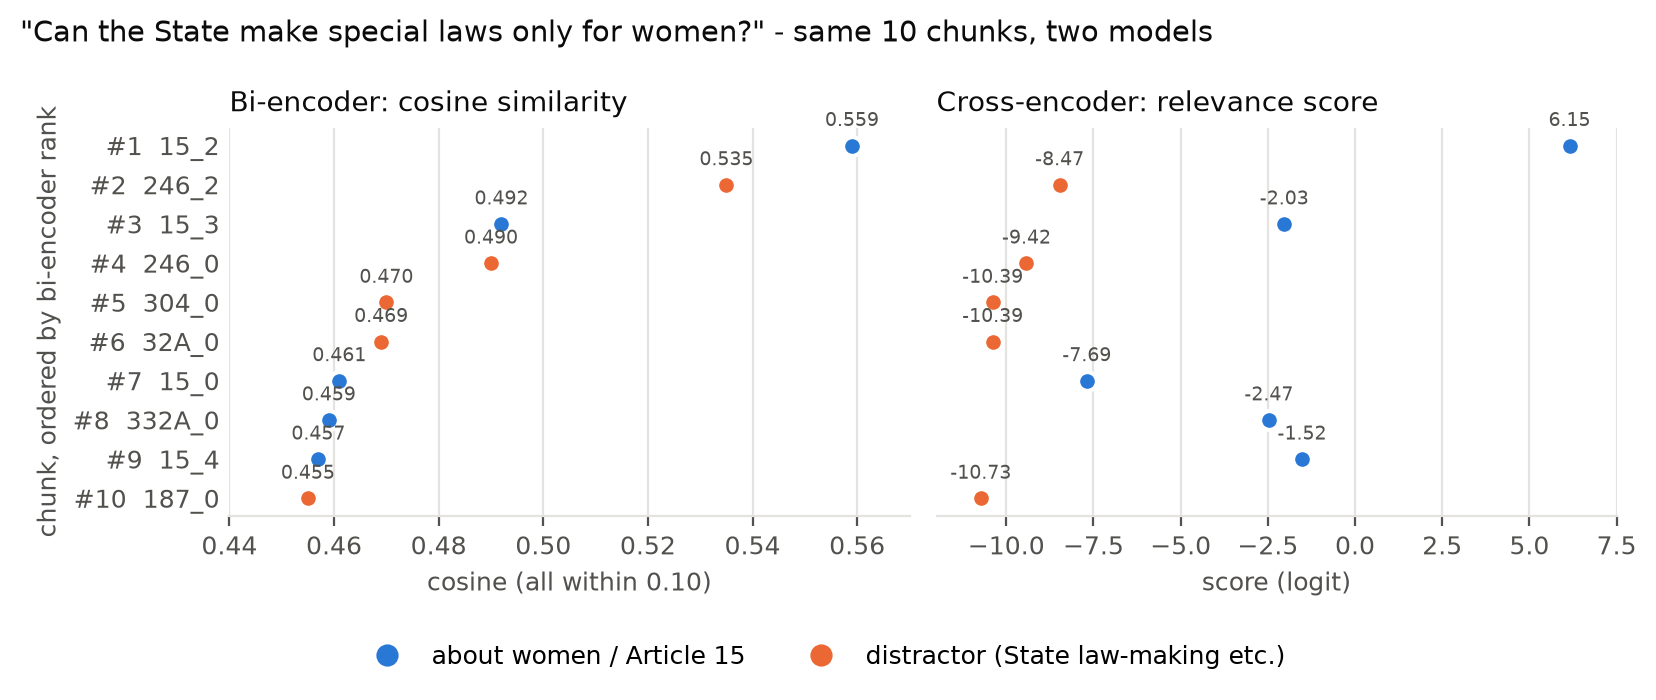
\includegraphics[width=\linewidth]{../figures/score_spread_women.png}
\captionof{figure}{The same 10 candidates scored by both models for the women query. Bi-encoder cosines are bunched within 0.10; cross-encoder scores spread from $+6.15$ to $-10.73$, demoting the State law-making distractors (Art.~246, 304, 187) but also the general rule 15(1) (\texttt{15\_0}).}\label{fig:spread}
\end{center}

\section{Failure-mode analysis}
The test set contains 52 queries across six categories, including questions about specific articles, exceptions, keyword traps, negation, synonyms, and information missing from the corpus. Each query has expected article(s) and a note about why retrieval might fail. We compared the top 10 chunks from both pipelines, checked the rank of the first relevant chunk, and compared the answers generated from the top 3. Since matching the right article does not always mean matching the right clause, the rescue cases were also checked at clause level. The categories and query results are listed in the separate results appendix (\texttt{results\_appendix.pdf}).

\par\medskip\noindent\begin{minipage}{\linewidth}\centering\small
\captionof{table}{Failure-mode categories.}\label{tab:categories}
\begin{tabularx}{\linewidth}{@{}>{\raggedright\arraybackslash}p{2.6cm}Yr@{}}\toprule
Category & What it tests & Queries\\\midrule
Document-specific & Questions about particular articles or clauses. These test whether retrieval can identify the correct provisions, especially when article numbers are involved. & 9\\
Exceptions & Questions about specific groups or exceptions to general rules. These test whether retrieval finds the specific provision instead of a general rule. & 10\\
Keyword traps & Articles with similar words but different meanings. These test whether retrieval finds the passage that actually answers the question. & 10\\
Negation & Questions about when rules do not apply or when certain actions are prohibited. These test whether retrieval can distinguish between positive and negative conditions. & 7\\
Out of corpus & Questions whose answers are absent from the document. The LLM should acknowledge that the provided context is insufficient rather than make up an answer. & 6\\
Synonyms & Questions that use different words from the document but have the same meaning. These test whether retrieval can handle differences in wording. & 10\\\midrule
\textbf{Total} & & \textbf{52}\\\bottomrule
\end{tabularx}
\end{minipage}\par\medskip

\subsection{Rank shifts and answers in the rescue cases}
In the rescue cases, re-ranking moved the relevant chunks into the top 3 and often improved the answer. For example, Article 361 moved from rank 7 to rank 1, allowing the second answer to explain the President's immunity and its exception. For caste discrimination, Article 15 moved from rank 6 to rank 1, so the second answer included the relevant prohibitions that the baseline missed. Article 370 also moved up, and the re-ranked answer included more of its clauses. However, retrieving the right chunk did not always guarantee a correct answer: both answers refused the question about the right to remain silent, showing that the LLM did not treat Article 20(3) (``compelled to be a witness against himself'') as a right to remain silent.

\par\medskip\noindent\begin{minipage}{\linewidth}\centering\small
\captionof{table}{Rescue cases: the answering chunk sat outside the baseline top 3 and the cross-encoder promoted it (clause-level).}\label{tab:rescue}
\begin{tabularx}{\linewidth}{@{}Y>{\raggedright\arraybackslash}p{2.9cm}>{\raggedright\arraybackslash}p{3.1cm}>{\raggedright\arraybackslash}p{3.4cm}@{}}\toprule
Query & Rank shift (bi$\to$ce) & Answer 1 (baseline) & Answer 2 (re-ranked)\\\midrule
Is the President immune from court proceedings? & 361\_1: 7$\to$1\newline 361\_0: 5$\to$2 & Refused (no Art.\ 361 in its top 3) & Correct: 361(1), 361(2) and the Art.\ 61 exception\\
Is caste discrimination illegal? & 15\_0: 6$\to$1\newline 15\_1: 10$\to$3 & Art.\ 15 title + special provisions; no 15(1)/(2) & Quotes 15(1) and 15(2)(a)/(b)\\
Does an accused person have the right to remain silent? & 20\_0: 6$\to$2 & Refused & Refused (chunk present)\\
What is Article 370? & 370\_0: 8$\to$2 & Only 370(3); 2 of 3 chunks unrelated & 370(1)(a), 370(1)(b) and 370(3)\\
Can the Vice-President act as President? & 65\_0: 4$\to$1 & Refused & Correct: vacancy 65(1); President unable to act 65(2)\\
Who appoints the judges of a High Court? & 217\_0: 7$\to$1 & Described additional/acting judges (Art.\ 224), not 217(1) & Correct: appointed by the President, 217(1)\\
Who is the supreme commander of the Defence Forces? & 53\_0: 4$\to$1 & Refused & Correct: vested in the President (Art.\ 53)\\
Can the Council of States be dissolved? & 83\_0: 6$\to$1 & Refused & Correct: not subject to dissolution, 83(1)\\\bottomrule
\end{tabularx}
\end{minipage}\par\medskip

\subsection{Where re-ranking did not help}
Re-ranking did not help every query. For the right to equality, Article 14 moved from rank 1 to rank 3. In the free-speech query, the top 3 missed the relevant clause on restrictions, and the second answer used provisions about speech in Parliament instead. Some questions also remained difficult because the wording differed from the document; for example, the Constitution uses “House of the People” rather than “Lok Sabha.” In other cases, the answer depended on a cross-reference or information outside the indexed text. Eight queries had no relevant chunk in the original top 10, so re-ranking could not recover them.

\subsection{Retrieval metrics}
On the 48 queries with an expected article, re-ranking improved Hit@3 from 0.69 to 0.81 and Precision@3 from 0.35 to 0.42. This means the top 3 contained relevant material more often; Hit@1 and MRR also increased slightly (0.60 to 0.62 and 0.67 to 0.71). Hit@10 stayed the same because both pipelines use the same initial set of 10 candidates. These scores are measured at article level, which can hide whether the exact clause was retrieved. The rescue cases show stronger gains at clause level, but they were selected because re-ranking helped and should not be treated as a general result.

\par\medskip\noindent\begin{minipage}{\linewidth}\centering\small
\captionof{table}{Retrieval metrics for the 48 queries with an expected article (article-level relevance). 6 of these queries were added after a search for rescue examples, which favours re-ranking. Per-query values: results appendix, Section C.}\label{tab:metrics}
\begin{tabular}{@{}lcc@{}}\toprule
Metric & Baseline & Re-ranked\\\midrule
Hit@1 & 0.60 & 0.62\\
Hit@3 & 0.69 & 0.81\\
Hit@10 & 0.83 & 0.83\\
Recall@3 & 0.64 & 0.76\\
Precision@3 & 0.35 & 0.42\\
MRR & 0.67 & 0.71\\
nDCG@10 & 0.69 & 0.73\\\midrule
First relevant chunk moved up / down & \multicolumn{2}{c}{8 / 8}\\\bottomrule
\end{tabular}
\end{minipage}\par\medskip

\section{Latency profiling}
Latency was measured on a laptop CPU, with the first model call excluded as warm-up. Retrieval and re-ranking were timed over 52 queries with three runs each; LLM timing was taken from saved calls. The bi-encoder took about 23 ms to retrieve 10 chunks from 1,035, while re-ranking those 10 took about 482 ms. So the retrieval stage became roughly 21 times slower. End-to-end median time increased from about 4.46 s to 4.97 s, around 11\%, because LLM generation still accounts for most of the total time.

\par\medskip\noindent\begin{minipage}{\linewidth}\centering\small
\captionof{table}{Latency per query (CPU; 52 queries $\times$ 3 runs after warm-up; LLM from 120 saved calls).}\label{tab:latency}
\begin{tabular}{@{}lrrr@{}}\toprule
Stage & Mean (ms) & Median (ms) & p95 (ms)\\\midrule
Bi-encoder retrieval (top 10 of 1,035) & 23.0 & 21.6 & 31.4\\
Cross-encoder re-ranking (10 pairs) & 482.0 & 506.1 & 595.8\\
Pipeline 1 retrieval total & 23.0 & 21.6 & 31.4\\
Pipeline 2 retrieval total (retrieval + re-rank) & 505.0 & 527.6 & 621.5\\
LLM generation (Gemini, per call) & 5147.8 & 4442.9 & 9910.5\\\bottomrule
\end{tabular}
\end{minipage}\par\medskip

\begin{center}
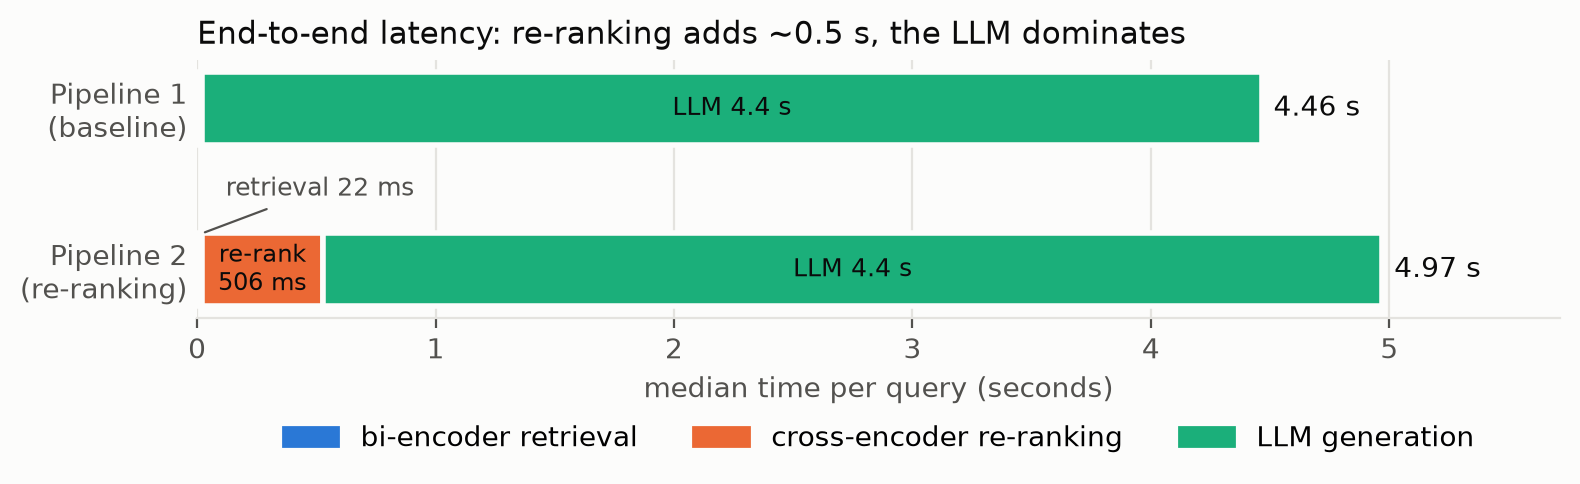
\includegraphics[width=0.9\linewidth]{../figures/latency_end_to_end.png}
\captionof{figure}{Median end-to-end time per query: Pipeline 1 $\approx$ 4.46\,s, Pipeline 2 $\approx$ 4.97\,s.}\label{fig:e2e}
\end{center}
\begin{center}
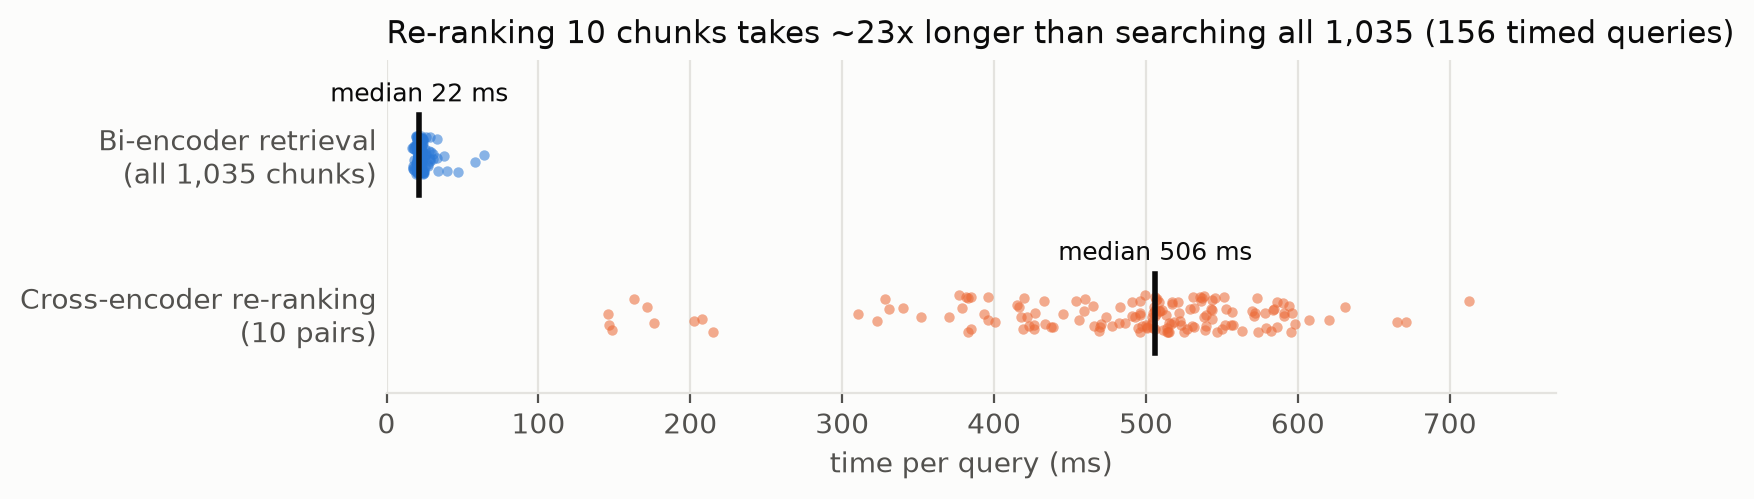
\includegraphics[width=0.9\linewidth]{../figures/latency_retrieval_vs_rerank.png}
\captionof{figure}{Bi-encoder retrieval vs.\ cross-encoder re-ranking for every timed query.}\label{fig:dist}
\end{center}

\section{Scaling: why not cross-encode everything?}
The cross-encoder must process each query and chunk together, so its score cannot be computed in advance. At about 48.2 ms per pair, scoring all 1,035 chunks would take roughly 50 seconds per query, compared with about half a second to re-rank only 10. The bi-encoder can store chunk embeddings ahead of time and quickly retrieve candidates; the cross-encoder then re-orders this smaller set more carefully. A larger candidate pool may recover more relevant chunks, but it also increases latency: in these tests, a top-20 pool would catch six of the eight missed queries, while a top-50 pool would catch all eight, at a higher cost.

\section{Limitations and possible extensions}
This version uses article text only, so questions that depend on schedules, appendices, or amendment footnotes may fail. Cross-references are not expanded, and the fallback splitting can sometimes cut a clause mid-sentence. The test set is also small, and article-level scoring does not always reflect clause-level relevance. A useful next step would be to combine dense retrieval with BM25, use a larger candidate pool, and expand cross-references. Query rewriting for terms such as “Lok Sabha” and better handling of footnotes could also improve results. A re-ranker trained on legal text may work better for this document.

\end{document}
